  \documentclass[11pt,fleqn]{article} %twocolumn,
  \usepackage{amsmath}
  \usepackage{amssymb}
  \usepackage{amsfonts}
  \usepackage{amsthm}
  \usepackage{eucal}
  \usepackage{graphicx}
  \usepackage{color}
  \usepackage{fancyhdr}
  \usepackage{geometry}
  %\usepackage{palatino}

  \usepackage{algorithm}
  \usepackage{algorithmic}
  \renewcommand{\algorithmicrequire}{\textbf{Input:~~}}
  \renewcommand{\algorithmicensure}{\textbf{Output:}}
  \allowdisplaybreaks

  \renewcommand{\baselinestretch}{1.1}
  \geometry{a4paper,headsep=7mm,hdivide={15mm,*,15mm},vdivide={20mm,*,15mm}}
    
  \renewcommand{\familydefault}{\sfdefault}
  \graphicspath{{pics/}{figs/}}

  \fancyhead[L]{\textit{MLR doc}---\today}
  \fancyhead[C]{}
  \fancyhead[R]{\thepage}
  \fancyfoot{}
  \pagestyle{fancy}

  \definecolor{bluecol}{rgb}{0,0,.5}
  \definecolor{greencol}{rgb}{0,.4,0}
  \usepackage[
    colorlinks,
    urlcolor=bluecol,
    citecolor=black,
    linkcolor=bluecol,
    pdfborder={0 0 0},
    pdfpagemode=UseOutlines
  ]{hyperref}

  \definecolor{codecol}{rgb}{.8,.8,.8}

  \usepackage{listings}
  \lstset{ %
    language=C,                % choose the language of the code
    basicstyle=\sf\footnotesize,       % the size of the fonts that are used for the code
    frame=none,                   % adds a frame around the code
    tabsize=4,                      % sets default tabsize to 2 spaces
    captionpos=b,                   % sets the caption-position to bottom
    texcl=true,
    mathescape=true,
    backgroundcolor=\color{codecol},
    escapechar=\%,
    columns=flexible,
    xleftmargin=1ex,
%    numbers=left, numberstyle=\footnotesize, stepnumber=1, numbersep=3ex
  }

  \usepackage{fancyvrb}
  \fvset{numbers=left,xleftmargin=5ex}
  \DefineShortVerb{\|}

  \makeatletter
  \newenvironment{code}{

    \begin{lrbox}{\@tempboxa}\footnotesize\begin{minipage}{.95\columnwidth}
  }{
    \end{minipage}\end{lrbox}%
    \colorbox[rgb]{.9,.9,.9}{\usebox{\@tempboxa}}

  }\makeatother



\newcommand{\T}{{\!\top\!}}
  \newcommand{\Id}{{\rm\bf I}}
\newcommand{\bi}{\begin{itemize}}
\newcommand{\ei}{\end{itemize}}

 
\title{The MLR Guide}
\author{Marc Toussaint}

\begin{document}
\maketitle

\centerline{Sources for this document: mlr/share/doc/guide.tex ~ \emph{Please contribute!}}

{\bigskip\hrule\vspace*{-2ex}\small\tableofcontents\medskip\hrule}

\section{Guide to Things}

This is the central hub for information. Goals of this document:
\begin{itemize}
\item Simply saying ``what is there'' and who could be asked to get further information.

\item The page should directly link to technical infos, be searchable, and be a kind of guide to beginners on where to start reading and find information.
\end{itemize}


\subsection{How to setup accounts, Ubuntu packages, external libs}

\begin{itemize}
\item You need at least an account on achtauge and redmine
  (https://maserati.mi.fu-berlin.de/redmine/projects/mlr)

\item The default directory layout:
\bi
\item |~/git/mlr| for your git repository
\item |~/lib| for your external lib installations
\ei

\item Create your git repository:
\begin{code}
\begin{verbatim}
cd ~/git
git clone ssh://<achtauge-user>@achtauge.imp.fu-berlin.de/mnt/data/git/share mlr
\end{verbatim}
\end{code}
See section \ref{secGit} on how to use git.

\item Install the following packages:
\begin{code}
\begin{verbatim}
liblapack-dev
freeglut3-dev
libqhull-dev
libf2c2-dev
libann-dev
libplib-dev
gnuplot
meld
libdc1394-22-dev
\end{verbatim}
\end{code}


\item For a full installation (e.g., interaction with the robot) one also
  needs the external libs
\begin{code}
\begin{verbatim}
cuda@
cudaSDK@
opencv-2.1@
ntcan@
schunkLWA@
schunkSDH-11-05-11@ 
\end{verbatim}
\end{code}

These are symbolic-linked in the |git/share/extern| directory. Call the
  |./LINK ~\lib| script to generate the relevant links.

Recently, opencv-2.3 has been used. When using Ubuntu, packages can be 
	obtained from |http://packages.ros.org/ros/ubuntu/|. For 
	convenience, the gpg-key is in the root folder.

\item TODO: In the future all external libs should be handled like
  |ODE_0.11|: minimal |GET/BUILD| script and .gitignore

\item Try 'make' in the |git/share| directory. If problems occur, try to
comment the following lines in the |src/MT/Makefile|:
\begin{code}
\begin{verbatim}
#FREEGLUT = 1
#ANN = 1
#LAPACK = 1
\end{verbatim}
\end{code}

This reduces functionality of the code, but should at least compile.

\item Generally, the |git/share/make-config| allows to set compile
options for all projects, the local Makefiles trigger these options by
defining 'ANN=1' or alike.

\item Try |test/array/x.exe|
\end{itemize}

\subsection{Guide to the robot hardware (Marc \& Stanio)}

\begin{itemize}
\item Startup hardware
\begin{itemize}
\item turn on robot
\item mlrMountHardware
\item mlrJoystick
\item mlrJoystick -openArm 1 -openHand 1 -openSkin 1
\end{itemize}

\item Debugging hardware:
\begin{itemize}
\item 09-testSchunkBasics
\item 09-testHandMotion
\item 09-testHandSense
\end{itemize}

\item Testing perception:
\begin{itemize}
\item 10-testEarlyVision
\item 10-testPerception
\end{itemize}

\item Learning about the control architecture:
\begin{itemize}
\item 10-miniExample (launches minimal set of Processes explicitly by hand)
\item RobotActionInterface (launches Processes using the RobotActionInterface)
\item 10-planningDemo
\end{itemize}
\end{itemize}


\subsection{Guide to BiROS (parallel processing architecture) (Marc)}


\subsubsection{Where to start learning}


\subsubsection{Status: the basic mechanisms in process.h are robust and reliable. }

\subsection{Guide to ORS (robot simulation data structures) (Marc)}

There are numerous robot simulation environments out there. Why
introduce a new one? Well, actually the aim of ORS is not to develop a
new full robot simulation environment. Instead, it aims to provide
basic data structures that help to link to existing external libraries
and algorithms together. In that way we can flexibly provide a
simulation environment with different features enabled by linking to
external libraries -- but always with the same basic interface as
provided by the ORS data structures.

The data structures are really simple and basic (see ors.h): Vector, Quaternion, Frame, Joint, Body, kinematic Graph -- that's basically it.

Beyond the data structures, ORS also implements two functional things:

\begin{itemize}
\item The jacobian (but that's trivial, given the kinematic graph)

\item So-called TaskVariables: These are very useful for designing motion
   control contraints (more precisely: cost terms for motion rate
   control or stochastic optimal control). The typical 'endeffector
   position' is only one type of task variable -- I've implemented
   many more (inclluding their Jacobians) which capture relative
   positioning, orientations, alignments, angles, between arbitrary
   frames of the kinematic graph; capturing collision costs, joint
   limit avoidance costs, etc etc. In practice, playing with task
   variables is often the core in designing elegant motions.

   ORS can currently link to the following external libraries:


\item SWIFT++ for collision (and proximity) detection. (Note: there is
   hardly any alternative out there to do proper proximity(!)
   detection. Bullet, ODE, SOLID, etc don't)

   (INSERT LIST OF ALTERNATIVE LIBS)

\item ODE for simple dynamic simulation including collision behavior
   (SWIFT++ only detects collisions, but doesn't simulate their
   effects)

\item OpenGL for display

\item blender (this is a bit outdated -- but I once wrote a python script
   to export/import blender geometries to ORS data structures)
\end{itemize}

Perhaps on the wishlist for ORS communication:
\begin{itemize}
\item OpenRAVE /  OpenGRASP

\item IBDS (perhaps much better dynamic simulation than ODE)

\item daVinci, bullet, OpenTissue

\item Yuval Tassas CapSim (new methods for EXACT contact simulation)
\end{itemize}

\subsubsection{Where to start learning about ORS}

\begin{itemize}
\item Robot lecture: the basic lecture on 3D geometry (to learn about my
conventions) and perhaps the lecture which introduces task variables
(and their Jacobians)

\item Have a look at ALL ors\_* test projects in the git repository --
they're really basic. Understand them all. The |ors_editor| is useful to
edit the ors-file describing geometries. Play with the |test.ors| file
while watching the effect in the window.

\item The ors doxygen.
\end{itemize}



\subsection{Guide to SOC \& AICO (Stochastic Optimal Control and motion
   planning routines) (Marc)}



\subsection{Guide to the Array class (the data structure most used throughout
   for vectors, matricies, tensors, lists, graphs, etc)}

This is a standard Array lib -- just like many others. (It actually
evolved from a lib started in Bochum, 15 years ago...) The main design
goals are: 

\begin{itemize}
\item compatibility with typical mathematical notation when coding
equations (That's in fact most important: It is curcial for us to be
able to code as directly as possible equations we've derived on
paper!)

\item compatibility with Matlab/Octave conventions (mostly...).

\item full transparacy and minimalism (for easier debugging),

\item Many features: unlimited rank tensors, fast memory handling, links
(by default) to LAPACK (@@is just as fast as any other
optimized matrix library), lists -- and everything implemented by only
a SINGLE basic class, not a whole lib of classes.
\end{itemize}

\subsubsection{Tip: Debugging with arrays}

If |*A.p@A.N|


\subsubsection{Important conventions}

\begin{itemize}
\item In all my code, a ``list'' is an array of pointers. Why? Years back
   I've implemented double linked lists (O(1) complexity for
   insertion/deletion) as was typically taught (back then) -- but in
   practise that's total nonsense. Insertion/deletion in a pointer
   array is also O(1). And array of point is so so much simpler and
   easier to debug.

   Convention: A ``ThingList'' is a typedef MT::Array<Thing*> !

\item Equally for graphs: A ``graph'' is a list of edges and a list of
   nodes! (What else?!) I've implemented basic graph template
   routines. They assume that the node type contains a list of
   in-edges, and a list of out-edges, and the edge type contains a
   pointer to the from-node and a pointer to the to-node.
\end{itemize}

\subsubsection{Where to start learning}

\begin{itemize}
\item Directly start looking at the 'array' test in the git
repository. Just by reading though all examples I think one learns
most.

\item The array doxygen.

\item The class has more features (functions) than one might think: I've
seem many students reimplementing routines that are actually already
there -- frankly I don't know how to avoid that.
\end{itemize}


\subsubsection{Future changes:}

\begin{itemize}
\item Instead of having explisit listX routines (for insertion, deletion,
   sort, etc) there will be a 'listMode' flag in the array class,
   indicating that this array is to be treated as a list of pointers.
\end{itemize}


\subsection{Guide to the visual perception software}

The current perception module does a very simple thing:
\begin{enumerate}
\item We have a left and right image. 'EarlyVision' is computing the
  HSV for these images. We assume to know a specific target $hsv^*\in[0,255]^3$
  values together standard deviations $\sigma_{hsv}\in[0,255]^3$. We compute
  the evidence $\theta_i = \exp(- (hsv_i-hsv^*)^2/\sigma_{hsv}^2)$ [sorry for
    sloppy notation] for each pixel $i$ in the left and right image.

\item Given $\theta_i$ in an image, we call OpenCV's flood-fill that finds
  the contour of the highest $\theta$-value region. Let's call the contour
  $\partial C$. (We do this for both images.)

\item Given the contour $\partial C$ we compute a distance-to-contour
  field/image: for each pixel $i$ we compute $d_i = \min_{j\in\partial C}
  \|i-j\|$ (using some OpenCV routine). We do this for both images. The
  image $d_i$ is a good potential cost function to let 2D contour
  models converge to the HSV contour.

\item We have three different parametric 2D contour models: 1) for a
  circle (1 parameter), 2) for a polygon with 6 vertices and parallel
  opposing edges (a bit like a hexagon, can fit any 2D-projected 3D
  box), 3) a contour model that corresponds to a 2D projected
  cylinder.

  We fit a contour model to the HSV contour by minimizing the sum of
  $d_i$ for all points on the contour model. We do this on both
  images. Fitting is done by gradient descent (RPROP). We get
  parameters of the 2D contours with sub-pixel accuracy.

\item Given the fitted 2D contours in the right and left image, we
  triangulate them. Giving us a 2D contour mapped into 3D space. From
  there it is trivial to fit a 3D ball, cylinder, or box.

\end{enumerate}

Note: It is not by accident that we stay 2D for until the last step:
in our experience it proved more robust to try to fit shapes/contours
in 2D first with as much accuracy as possible before triangulating.



\subsection{Guide to further existing software}

\subsubsection{Optimization methods (Marc)}

There are quite a bit of generic optimization methods implemented --
but not well documented/organized yet:

\begin{itemize}
\item Rprop (best gradient descent method)

\item GaussNewton

\item CMA

\item Some Genetic \& Evolutionary Algorithms (e.g., similar to CMA)
\end{itemize}

Ask Marc.



\subsubsection{Inference and Machine Learning methods (Marc)}

We have probabilistic inference code (infer lib) and also basic
Machine Learning methods (as introduced in the ML lecture). Ask Marc.

\begin{itemize}
\item Gaussian Processes

\item ridge regression, logistic regression, etc

\item MDPs, POMDPs
\end{itemize}



\subsubsection{Computer Vision methods (Marc)}

LINK to my notes on the CV system


\subsubsection{Robotics algorithms (Nikolay \& Marc)}

\begin{itemize}
\item RRTs

\item Trajectory Prediction

\item etc
\end{itemize}



\subsubsection{Relational RL (Tobias)}

\begin{itemize}
\item Robot Manipulation Simulator: http://userpage.fu-berlin.de/tlang/RMSim/

\item libPRADA, a library for relational planning and rule learning: http://userpage.fu-berlin.de/tlang/prada/
\end{itemize}


\subsubsection{coding utilities}

\begin{itemize}
\item String class

\item Parameters read from cmd line or config file

\item plotting in opengl \& gnuplot

\item opengl using freeglut, fltk or qt
\end{itemize}









\section{How To do things}


\subsection{git workflow}\label{secGit}

Most likely (I would wonder if not) the git man pages are installed
together with the git binaries in your distribution. The fastest way to
check the syntax or parameters of a git subcommand are the man pages. 

As a preliminary to using git, please take an hour to read the two
tutorials on git provided in the man pages. In your terminal write
|man gittutorial|. When done with it read on with %
%
|man gittutorial-2|. Depending on your background and experience
with other revision control systems there might be better approaches to
introduce git, but at any rate, these two tutorials give basic
insight into git's concepts. For deeper understanding %
%
|man gitcore-tutorial| is your friend.

Usually, |git foo help| is synonym for |man git foo|.

\begin{code}
\begin{verbatim}
git clone ssh://<achtauge-user>@achtauge.imp.fu-berlin.de/mnt/data/git/share mlr
git config --global diff.external git-diff.sh
git config --global push.default tracking

git status
git diff
git add|mv|rm|... <files>
git commit -am 'message'  (or --all --message 'message')
git pull --all
git push --all

git branch -a
// overview over all branches and configs for push and pull
git remote show achtauge
git checkout <branch>
git branch <new-branch>
git branch --track <new-branch> <remote-branch>
// set branch to pull from some remote branch
git branch --set-upstream <existing-branch> <remote-branch-to-be-tracked>
// Example: git branch --set-upstream branch123 origin/branch123
git merge <other-branch>

.gitignore
git update-index --assume-unchanged <files>
\end{verbatim}
\end{code}

with a git-diff.sh file (in your local bin)
\begin{code}
\begin{verbatim}
#!/bin/bash
/usr/bin/meld "$2" "$5" > /dev/null 2>&1
\end{verbatim}
\end{code}

Some other contribution to the git cheat sheet:


\begin{itemize}


\item{init} 

- |git init|  just inits the |$PWD|, nothing added, nothing

- create central repo for current development\begin{enumerate}
	
	\item at home, |cd ~/dev/mpcdzen|, |git init|
	\item |git add mpcdzen.sh mpcdzen.conf|  
	\item |git commit -m initial|
	\item |ssh my.server.there| go to where my 'central' repos are.
	\item |cd ~/gitrepos/; git clone --bare  ssh://my.home.here/home/me/dev/mpcdzen|
	\item everywhere: |git clone ssh://my.home.here/home/me/dev/mpcdzen| \end{enumerate}

- when cloning on the same machine:
  %
  |git clone --bare --no-hardlinks -l ~/dev/mpcdzen|  can be helpful



\item{commit}

- |git add -u ../path/| : add all *tracked* files under path

- |git add ../path/| : add *all* files under path to staging area

- |git commit -a | : add all modified tracked files from the *whole
  working copy* and commit
  	

\item{diff}
  	
- |git diff| : how current files and HEAD differ

- |git diff --cached | : diff staged files against HEAD


\item{status}

- |git status| : list staged, modified tracked, untracked files

- if |file| is not tracked you can use .gitignore or .git/info/exclude
  to tell git not to take care of it. If it is already tracked, this is
  the way to say the same: |git update-index --assume-unchanged ../file|  

\item{remote}

- |git add remote mhmgr ssh://my.homemachine/git/repo| kinda introduces
  my home machine's repo to this one. Then, |git fetch mhmgr| and I'm
  set to go for comparing, merging etc.

\item{refs' naming}

- |HEAD^| addresses the parent of |HEAD|, e.g., assuming I've
  merged 2 branches and committed 3 times on the current branch, 
  %
  |git show HEAD^^^2| shows the second branch before merging. In
  other words, direct after merge and commit, the parents of HEAD are
  |HEAD^1|  and |HEAD^2|  
   
   illustration from man git-rev-parse:
   
   \begin{code} \begin{verbatim}
           G   H   I   J
            \ /     \ /
             D   E   F
              \  |  / \
               \ | /   |
                \|/    |
                 B     C
                  \   /
                   \ /
                    A

           A =      = A^0
           B = A^   = A^1     = A~1
           C = A^2  = A^2
           D = A^^  = A^1^1   = A~2
           E = B^2  = A^^2
           F = B^3  = A^^3
           G = A^^^ = A^1^1^1 = A~3
           H = D^2  = B^^2    = A^^^2  = A~2^2
           I = F^   = B^3^    = A^^3^
           J = F^2  = B^3^2   = A^^3^2

\end{verbatim} \end{code}

\item{fork file with history}

git doesn't have cp subcommand. The equivalent to \verb+git cp a b+ is 
\begin{code}\begin{verbatim}
cp a b
git add b
\end{verbatim} \end{code}

git doesn;t have means to track hisory of files. It tracks |blobs|.
See gitcore-tutorial for details. The history is available in, e.g.
%
|git log|, through |-C| option (Then git tries to find copies.
It is good idea to commit forked files together -- then -C has clue
where to search. If you would not, |-C -C| (double -C) or
--find-copies-harder (or so) does the trick)
http://www.gelato.unsw.edu.au/archives/git/0612/34502.html

\end{itemize}

\subsection{Setting Up GIT Server to Maserati}

First type
\begin{verbatim}
git remote -v 
\end{verbatim}
to see which git server you use. In case it is not maserati you should change this!

\begin{itemize}
\item in your web browser go to
\begin{verbatim}
https://maserati.mi.fu-berlin.de/redmine/
\end{verbatim}
and login with your account on maserati

\item  browse to \textit{Public keys,New public key} and click \textit{ new value}  \\
create a sshkey in the webpage, e.g. by copying some ssh file from your computer, here we use gedit for example:
 \begin{verbatim}
 cd .ssh 
 gedit id_rsa.pub
 \end{verbatim} 
 copy everything after the 'ssh-rsa' string for key value and activate it on the server
\item type in your computer to add maserati as server:
 \begin{verbatim}
git remote add maserati git@maserati.mi.fu-berlin.de:mlr 
 \end{verbatim}
\item 
go to your main git folder and type
 \begin{verbatim}
gedit .git/config
 \end{verbatim}
then change all your remotes to maserati, remove any old/conflicting origins entries, it should look like this:
 \begin{verbatim}
[branch "master"]
	remote = maserati
	merge = refs/heads/master
[remote "maserati"]
	url = git@maserati.mi.fu-berlin.de:mlr
	fetch = +refs/heads/*:refs/remotes/maserati/*
\end{verbatim}
	\end{itemize}

\subsection{svn workflow}

\begin{code}
\begin{verbatim}
svn co --username=<YOUR ZEDAT LOGIN> --password=<YOUR ZEDAT PW> https://svn.imp.fu-berlin.de/mlr
svn add|del|mv <files>
svn up
svn commit -m 'message'
\end{verbatim}
\end{code}



\subsection{LaTeX Conventions}

\subsubsection{References}

\begin{code}
\begin{verbatim}
\usepackage[round]{natbib}
\bibliographystyle{abbrvnat}
\end{verbatim}
\end{code}

\subsubsection{Generating figures / graphical models}

\begin{enumerate}

\item Use Inkscape. See the example mdp.svg in the pics path (note
the |\graphicspath{{pics/}}| command):

\centerline{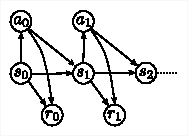
\includegraphics[scale=.5]{mdp}}


  Use the 'Tex Text' plugin. Use layers to generate animations. Use
  `save a copy' to export as pdf (potentially with some layers
  switched off)

\item Use xfig with 'special tag' text. Use the following fig2pdf script to
  convert:

\begin{code}
\begin{verbatim}
rm -f $1.pdf
rm -f $1.tex
fig2dev -Lpdftex -p $* $1.fig $1.pdf
fig2dev -Lpstex_t -p $* $1.fig $1.tex

cp $HOME/write/tex/figs/header.tex z.tex
printf "%s\n" "\\input{$1.tex}" >> z.tex
printf "%s\n" "\\end{document}" >> z.tex
more z.tex
pdflatex z.tex
pdfcrop z.pdf $1.pdf
\end{verbatim}
\end{code}
\end{enumerate}



\subsubsection{Space tricks}

Be creating in using any of the following\\
\begin{code}
\begin{verbatim}
  \renewcommand{\baselinestretch}{.98}
  \renewcommand{\arraystretch}{1.2}
  \renewcommand{\textfloatsep}{3ex}
  \renewcommand{\floatpagefraction}{.6}
  \renewcommand{\dblfloatpagefraction}{.6}
  \setlength{\mathindent}{2.5em}
  \setlength{\jot}{0pt} %zwischen den math zeilen
  \setlength{\abovedisplayskip}{-10pt}
  \setlength{\belowdisplayskip}{-10pt}
  \setlength{\mathsurround}{-10pt}
  \renewcommand{\floatsep}{-1ex}
  \renewcommand{\topfraction}{1}
  \renewcommand{\bottomfraction}{1}
  \renewcommand{\textfraction}{0}
  \columnsep 5ex
  \parindent 3ex
  \parskip 1ex
\end{verbatim}
\end{code}

Or more compact lists:\\
\begin{code}
\begin{verbatim}
\begin{list}{--}{\leftmargin4ex \rightmargin0ex \labelsep1ex
  \labelwidth2ex \topsep-\parskip \parsep.5ex \itemsep0pt}
\item ...
\item ...
\end{list}
\end{verbatim}
\end{code}

The |list| parameter documentation:\\
\begin{code}
\begin{verbatim}
   * \topsep amount of extra vertical space at top of list
   * \partopsep extra length at top if environment is prececed by a blank line (it should be a rubber length)
   * \itemsep amount of extra vertical space between items
   * \parsep amount of vertical space between paragraphs within an item
   * \leftmargin horizontal distance between the left margins of the environment and the list; must be nonnegative
   * \rightmargin horizontal distance betwen the right margins of the enviroment and the list; must be nonnegative
   * \listparindent amount of extra space for paragraph indent after the first in an item; can be negative
   * \itemindent indentation of first line of an item; can be negative
   * \labelsep separation between end of the box containing the label and the text of the first line of an item
   * \labelwidth normal width of the box containing the label; if the actual label is bigger, the natural width is used, extending into the space for the first line of the item's text
   * \makelabel{label} generates the label printed by the \item command
\end{verbatim}
\end{code}

\subsubsection{Generating pseudo code}

See Algorithm \ref{algGN}

\begin{algorithm}[ht]
\caption{Gauss-Newton with adaptive Levenberg Marquardt parameter}
\label{algGN}
\begin{algorithmic}[1]\small
\REQUIRE start point $x$, tolerance $\delta$, routines for $x \mapsto
  (\phi(x), J(x))$
\ENSURE converged point $x$
\STATE initialize $\lambda=1$
\STATE compute $(\phi, J)$ at $x$ and $l=\phi^\T \phi$
\REPEAT
\STATE\label{redo} compute $\Delta$ to solve $(J^\T J +\lambda \Id)~ \Delta = - \sum
J^\T \phi$
\STATE $x' \gets x + \Delta$
\STATE compute $(\phi, J)$ at $x'$ and $l'=\phi^\T \phi$
\IF{$l'>l$}
\STATE $\lambda \gets 2\lambda$
\ELSE
\STATE $\lambda \gets 0.8\lambda$
\STATE $x \gets x'$
\ENDIF
\UNTIL $\|\Delta\| < \delta$
\end{algorithmic}
\end{algorithm}


%%%%%%%%%%%%%%%%%%%%%%%%%%%%%%%%%%%%%%%%%%%%%%%%%%%%%%%%%%%%%%%%%%%%%%%%%%%%%%%%

\subsection{Coding Conventions}

\begin{enumerate}
\item Take the Google C++ style as default:
  \url{http://google-styleguide.googlecode.com/svn/trunk/cppguide.xml}.
  The rules below overwrite Google conventions.

\item Output parameters before input parameters in function declarations.

\item Naming convention |name_of_a_routine(ouput,input);| is
  perhaps better than my old |nameOfARoutine(..);| style.

\item Make headers as clean and short and concise as possible!

\item Try to avoid |#includes| in header files as much as possible!!
  In particular, when a class's methods require an external library;
  this external library should be included only in the cpp-file.

 $\to$ In particular, try to avoid |#includes <external_lib>| in headers!! (I
 tried to get rid of them as much as possible in all my *.h)

\item Try to avoid |#includes| in header files as much as possible!!
  If
  you think the class needs to contain members/data structures defined
  in an external library and therefore you need to include its header
  in your header --- that's often not true. Instead, hide all members
  in a \emph{``hidden self''}:

Bad example:

\begin{code}
\begin{verbatim}
//h-file:
#include <OpenCV> //BAD

struct MyClass{
  OpenCV_DataStructure data;
};
\end{verbatim}
\end{code}

Good example:

\begin{code}
\begin{verbatim}
//h-file:

struct sMyClass; //forward declaration of a 'hidden self' that will
contain all members hidden from the header

struct MyClass{
  sMyClass *s; //maybe call it 'self' instead
};

//cpp-file:
#include <OpenCV> //GOOD

struct sMyClass{
  OpenCV_DataStructure data;
};

MyClass::MyClass(){
  s = new sMyClass;
}
\end{verbatim}
\end{code}

\item Move documentation to cpp files. Advantages: You can write as
  long and lengthy documentation as you want without destroying the
  beauty of the header. Doxygen will compile this without problem to
  provide a nice documentation. If people want to read the
  documentation from source directly---it's not much of a hassle to
  find the definition in the cpp file.


\item Never ever use |#ifdef| directives in a header file if this
  influences definition of classes, especially which members (and
  'size') a class has!

  The following debugging horror may happen: You define a class to
  have different members depending on a compiler flag. You compile
  your library with some compiler flags. The user includes your header
  with other compiler flags. Everything seems to compile and link
  fine. But when the user accesses members of the class, he actually
  refers to different memory addesses as your routines in your
  library.

  Therefore try to avoid |#ifdefs| in headers as much as possible! Move
  them to the cpp file!

\item If you don't have a preferred IDE, use kdevelop.

  K\&R formatting conventions!

  Editing: use spaces instead of tabs. 2 characters. Identation with 2
  characters.

  Keys: F10,11,12: step, step in, step out, F9: toggle break\\
  F8 clean, F7 build, F5 debug run, CtrlF5 run, F6 continue


\item fltk lists their conventions -- I like them, also
  their style of formatting and their makefile conventions

\end{enumerate}


\section{Points to improve the code}

\begin{description}
\item[Penetrating collisions] The way penetrating collisions are
handled is really not nice |ors_swift.cpp:318|. What should ideally
happen: find the two points on the meshes that penetrate most, set $d$
as their negative distance, and the penetration normal aligned with
their distance. What happens now: set the distance $d=0$ and set the
normal align with the shape centers. The problem: the collision
gradient is not really correct.

What to do: Actually most other collision libs focus on penetration
(bullet/ode/solid), only SWIFT focusses on distance queries. What one
would have to do, call one of these other collision libs to compute
the most-penetrating two points of convex shapes.


\end{description}

\subsection{Marc's older notes for code}

\begin{enumerate}

\item Processes may not access MT.cfg in their step routine (open() is
  acceptable, but still not optimal).

  Instead, if necessary, parameters need to be made a proper
  variable. A special gui process offers a way to modify the variable
  online by the user.

\item The |Lock| (from |process_internal.h|) should actually not be used. The
  fact that it is used right now shows bad programming: It is always
  used when one process (or main loop) accesses directly another
  process instead of via a variable. Change that!

\item Make some central |ors| variable, or so, from which
  processes can update their ors-structure. Perhaps that needs
  some signalling -- currently this orsCopyStuff after the
  connectivity is changed (object glued to hand/released) is not at all clean
  (related to point above).

\item The motion planners so far only optimize the next to go
  motion. Ideally there should be parallel planners optimizing already
  future motions $\to$ Dmitry's keyframe approach.

\item Make a Variable out of the TaskVariableList!! 

\item All variables should have setters and getters of the format

|arr& get_qreal(Process*);|

|void set_qreal(Process*,const arr&);|

These throw errors if called from a process that hasn't locked the
variable or is a 'set' is called in readLock.

\item robot.cpp:281: read the current state in the schunk.open() routine!
not here!

\item remove setting accelerations in each step of schunk hand motion

-- use radians (SDH constructor) out of the box

-- set and get velocites with one function call to schunk lib

\item SOC: make consistent to what is written in the TOMSY document

\item GRASP HEURISTICS: 1) Instead of conditioning velocities for lifting
  and placing, condition positions directly. 2) For grasp-approach:
  instead of conditioning only final position, condition on an
  approach position-profile: namely in the reference frame
  object-relative-to-hand. In both cases, use sinus position profiles?

\end{enumerate}



\subsection{Nikolay's ideas for vision}
\begin{enumerate}

\item improve quality of color segmentation, while staying cheap
  computationally: learn a discriminative classifier $f(x)$ to
  separate by HSV color pixel of interest $x$ from background

\item to get an intuitive interface without too much program overhead:
  create mask of desired discrimination as an image and train
  classifier in external program (matlab or C++), to output model
  parameters

\item use a mixture of $k$ Gaussians for the activation of pixel $x$
  in HSV space: $f(x) = \sum_k \alpha_k exp(- \frac{\|c_k -
    x\|^2}{\sigma_k})$ , probably 2 Gaussians are already more than
  enough, the current code is equivalent to $k=1$ single Gaussian

\item just load parameters of trained Gaussian mixture and incorporate
  in earlyvisionmodule.step(): for each gaussian $k$ we will calculate
  one response image and than sum them, to use the existing data
  structures make $\sum_k \alpha_k = 1$

\item optionally, use RGB space in addition to HSV space

\item use the above techniques for the LEDtracker... should simplify
  dealing with reflections

\item For an example how an image interface can be useful to define
  labels for training discriminative segmentation: few brush strokes
  are enough to define regions of foreground and background see
  frogsegment.jpg, (algorithm implemented by me in matlab)
\end{enumerate}


\end{document}

